\chapter{Execution}\label{sec:Execution}
To start a Varroa test the user needs to start a Commander and at least one Agent.
The Agents periodically try to establish a connection to the Commander.
Once all Agents are connected the execution of the scenario starts.
\textsl{}
\section{Commander}
\begin{figure}[H]
	\begin{center}
	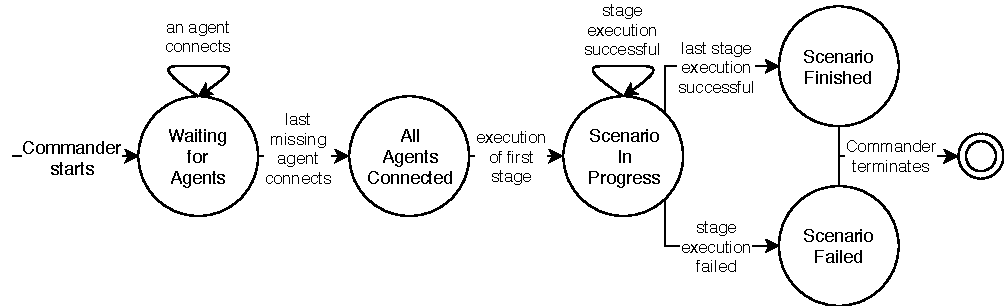
\includegraphics[scale=0.9]{Resources/PDF/CommanderStates}
	\caption{Commander States}
	\label{pic:CommanderStates}
	\end{center}
\end{figure}
After starting a Varroa Instance that is configured as a Commander (see \ref{sec:commanderConfig}) it waits for the Agents to connect.
Until all Agents are successfully connected the Commander remains in the \emph{Waiting for Agents} state.
As the last missing Agent connects the Commander switches its state to \emph{All Agents Connected}.
Then it parses the Scenario's XML. As soon is this is done, the Commander starts to distribute the Scenario's first stage to the Agents.
In doing so the Commander changes its state to \emph{Scenario in Progress}.
It remains in this state until all stages are executed successfully and then transfers its state into \emph{Scenario Finished}.
Contrary to this case a faulty execution of a stage results in the failure of the whole Scenario, logically the Commanders state is then \emph{Scenario Failed}.
To allow better comprehension figure \ref{pic:CommanderStates} illustrates this process.

\subsection{Agent}
\begin{figure}[H]
	\begin{center}
	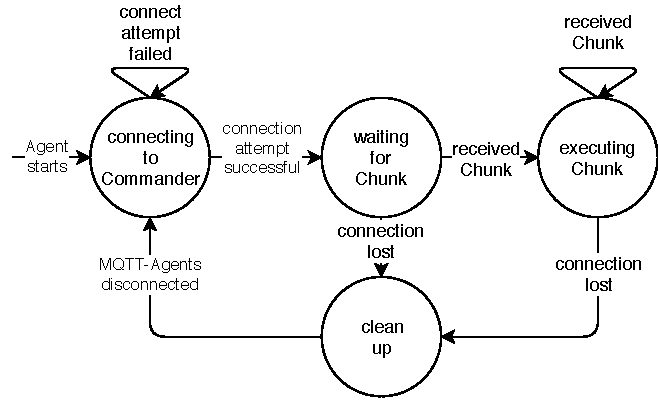
\includegraphics[scale=0.9]{Resources/PDF/AgentStates}
	\caption{Agent States}
	\label{pic:AgentStates}
	\end{center}
\end{figure}
Upon starting a Varroa Instance as an Agent, it tries to connect to the configured Commander (see \ref{sec:agentConfig}).
It periodically attempts to establish the connection until it succeeds.
Then it waits for incoming Chunks from the Commander and executes them, implementing the handshake protocol introduced in \ref{sec:chunkDistribution}.
The Agent continues doing so until it loses the connection to the Commander.\\
In contrast to the Commander the Agents life-cycle does not stop after the execution of a Scenario.
Because of this the user only needs to restart the Commander to execute another Scenario.
For better understanding of the temporal processes the just explained concepts are illustrated in figure \ref{pic:AgentStates}.

\section{Configuration}
\subsection{Commander}\label{sec:commanderConfig}
\begin{lstlisting}[caption={Commander XML configuration}, captionpos=b, label={lst:commanderConfig}, language=XML]
<varroa>
    <commander>
		<bind-host>192.127.0.1</bind-host>
        <bind-port>12345</bind-port>
        <amount-agents>3</amount-agents>
    </commander>
</varroa>
\end{lstlisting}
\begin{itemize}
	\item \textbf{bind-host:} specifies the Address the Commander binds to
	\item \textbf{bind-port:} specifies the port the Commander binds to for waiting for Agent connections
	\item \textbf{amount-agents:} specifies the amount of Agents that connect to the Commander
\end{itemize}

\subsection{Agent}\label{sec:agentConfig}
\begin{lstlisting}[caption={Agent XML configuration}, captionpos=b, label={lst:agentConfig}, language=XML]
<varroa>
    <agent>
		<commander-host>192.127.0.1</commander-host>
        <commander-port>12345</commander-port>
        <local-port>23458</local-port>
		<commander-retry-interval>10</commander-retry-interval>
    </agent>
</varroa>
\end{lstlisting}
\begin{itemize}
	\item \textbf{commander-port:} specifies the port of the Commander
	\item \textbf{commander-host:} specifies the Address of the Commander
	\item \textbf{local-port:} specifies the local port the Agent uses for the outgoing connection to the Commander %TODO must be different on every Agent
	\item \textbf{commander-retry-interval:} the time interval in which Agents try to connect to the Commander
\end{itemize}